% Zeker nog library voor afstand nog
\chapter{Implementatie} \label{chap:implementatie}
De eerste stap in deze thesis was het onderzoeken van hoe Android omgaat met locatiegegevens en het implementeren van deze functionaliteit in een testapplicatie. Zodra deze applicatie functioneel was, werden de eerste preliminaire testen uitgevoerd en werd de nuttige code afgesplitst om de basis te vormen van de Android-library.
\section{Overzicht library}
De structuur van de library is weergegeven in Figuur~\ref{fig:uml_library}. Het merendeel van de functionaliteit is ondergebracht in de klasse \texttt{LocationManager}, die fungeert als het centrale beheerpunt voor locatieverzameling. De klasse \texttt{LocationWorker} vormt de implementatie die vereist is om de WorkManager te benutten voor achtergrondtaken. Daarnaast biedt de interface \texttt{LocationObfuscator} een abstractielaag waarmee ontwikkelaars eigen obfuscatie-algoritmes kunnen implementeren.
\begin{figure}
    \centering
    \includesvg[width=0.75\textwidth]{images/uml.svg}
    \caption{Klasse diagram van de library}
    \label{fig:uml_library}
\end{figure}
\subsection{Locatie tracking}
Het centrale onderdeel van de library, namelijk de locatieverzameling, wordt beheerd door de \texttt{LocationManager}, die fungeert als het centrale aanspreekpunt. Deze klasse beheert alle benodigde variabelen voor locatieverzameling en biedt setters met ingebouwde validaties om de stabiliteit te waarborgen. Variabelen die specifiek zijn voor obfuscatie worden echter beheerd door de obfuscator zelf, aangezien deze buiten de verantwoordelijkheid van de \texttt{LocationManager} vallen.

\subsubsection{Background en foreground services}
Voordat locaties verzameld kunnen worden, moeten enkele beperkingen in acht worden genomen. Allereerst mogen locaties niet worden opgevraagd in dezelfde thread als de activity waarmee de gebruiker interacteert. 
Zelfs als dit in een aparte thread vanuit de hoofdactivity wordt opgestart. Is dit geen oplossing voor permanente locatieverzameling want Android zal deze beëindigen vanwege de strikte beperkingen op services wanneer de activity wordt gestopt of vernietigd.

Om taken uit te voeren wanneer de hoofdactivity niet actief is, kan gebruik worden gemaakt van foreground services of background tasks. Voor deze library is gekozen voor de WorkManager, vanwege de flexibiliteit en betrouwbaarheid die deze biedt. De WorkManager kan zowel functioneren als een foreground service als een periodieke background task, waardoor de zelfde klasse die de Worker van WorkManager implementeert kan gebruikt worden voor beide.

\paragraph{Foreground services}
Een foreground service wordt gebruikt om langdurige taken uit te voeren die een hogere prioriteit vereisen. Om een service als foreground service te configureren, moet in de hoofdactiviteit een notificatiekanaal worden aangemaakt. Dit notificatiekanaal zorgt ervoor dat de gebruiker visueel geïnformeerd wordt over de achtergrondactiviteit. 
Nadat het notificatiekanaal is aangemaakt, kan de Worker, een klasse die de vereiste interface van de WorkManager implementeert, een notificatie genereren en weergeven.
Dit gebeurt als volgt in de \texttt{LocationManager}, zoals weergegeven in onderstaande code, die een referentie heeft naar de hoofdactiviteit. De \texttt{LocationManager} maakt een notificatiekanaal aan met \texttt{IMPORTANCE\_LOW} om de gebruiker zo min mogelijk te storen.
\begin{minted}[breaklines]{java}
private fun setupNotificationChannel() {
    val channelId = "locationTrackingChannel"
    val channelName = "Location Tracking"
    val channelDescription = "Location tracking is active"
    val notificationManager =
        activity.getSystemService(NOTIFICATION_SERVICE) as NotificationManager

    // Create notification channel if not already created
    val channel =
        NotificationChannel(channelId, channelName, NotificationManager.IMPORTANCE_LOW).apply {
            description = channelDescription
        }
    notificationManager.createNotificationChannel(channel)
}
\end{minted}
Dan kan de LocationWorker ingrijpen op dit notificatiekanaal door dezelfde ID aan te spreken. De nodige info is een notificatie voor de foregroundInfo, zodat Android weet waarvoor de notificatie bedoeld is. De implementatie Hiervoor is te zien in onderstaande code.
\begin{minted}[breaklines]{java}
val notification =
    NotificationCompat.Builder(applicationContext, "locationTrackingChannel")
        .setContentTitle("Location Tracking")
        .setTicker("Location Tracking")
        .setContentText("Tracking your location in the background")
        .setSmallIcon(R.drawable.ic_launcher_background)
        .setOngoing(true)
        .build()

val foregroundInfo =
    ForegroundInfo(1001, notification, ServiceInfo.FOREGROUND_SERVICE_TYPE_LOCATION)
setForegroundAsync(foregroundInfo)
\end{minted}

Zodra de notificatie is geactiveerd, kan de Worker ononderbroken blijven werken totdat deze zichzelf beëindigt of totdat de functie \texttt{cancelUniqueWork} van de WorkManager wordt aangeroepen vanuit de hoofdactivity. Deze aanpak zorgt ervoor dat de taken betrouwbaar en efficiënt worden uitgevoerd, zelfs wanneer de applicatie zich niet op de voorgrond bevindt.

\paragraph{Background tasks}
Wanneer een visuele indicatie van achtergrondactiviteit niet vereist of mogelijk is, kan gebruik worden gemaakt van periodieke taken. Historisch gezien werd hiervoor de \texttt{AlarmManager} gebruikt, die functioneerde als een soort cron job in Linux. Echter, vanwege strengere beperkingen op maximale duur en frequentie, is deze aanpak minder geschikt geworden.

De WorkManager biedt een modern en aanbevolen alternatief voor het uitvoeren van periodieke taken. Er zijn echter enkele beperkingen: taken kunnen maximaal één keer per 15 minuten worden uitgevoerd en mogen niet langer dan 10 minuten actief zijn. Ondanks deze restricties is de WorkManager robuust, energiezuinig en goed geïntegreerd met het Android-platform, waardoor achtergrondprocessen betrouwbaar beheerd kunnen worden. Qua implementatie wordt dezelfde codebasis gebruikt als voor de foreground service, maar zonder het opzetten van het notificatiekanaal zoals hierboven beschreven.

\paragraph{Integratie in de library}
Doordat de WorkManager beide vereisten kan afhandelen, is er slechts één klasse nodig die zowel foreground services als periodieke taken implementeert. Deze klasse, die de \texttt{Worker}-interface implementeert, bevat tevens de \texttt{LocationCallback} die vereist is voor de \texttt{FusedLocationProvider}. Deze callback speelt alle resultaten direct door naar de \texttt{LocationManager}, die deze resultaten vervolgens verwerkt volgens de ingestelde configuratie. Deze aanpak minimaliseert de complexiteit en verhoogt de herbruikbaarheid van de code.

Een bijkomende reden om de \texttt{LocationManager} als een Singleton te implementeren, is de beperking van de LocationWorker om complexe structuren of referenties door te geven. Zo is de initialisatie van een Worker beperkt tot primitieve datatypes. Hierdoor kan er geen referentie doorgegeven worden naar een stop signaal. Want door gebruik te maken van een Singleton-patroon kan de LocationWorker de \texttt{LocationManager} initialiseren en een referentie behouden naar diens variabelen. Zo bevat de \texttt{LocationManager} bijvoorbeeld een boolean genaamd \texttt{running}, waarmee kan worden aangegeven of de locatieverzameling actief is. Indien de locatieverzameling wordt stopgezet, kan de LocationWorker deze status uitlezen en zichzelf correct beëindigen.
\subsubsection{Permissies}
Een voordeel van Android is sandboxing, waardoor alles waar de applicatie probeert toegang tot te krijgen gemonitord kan worden. 
Hierdoor is het noodzakelijk dat de applicatie expliciet toestemming vraagt voor bepaalde functionaliteiten; indien deze toestemming niet wordt verkregen, zal de applicatie bij een toegangsverzoek crashen. Alle benodigde permissies horen ook in het manifestbestand vermeld te worden.
Dit manifestbestand is vergelijkbaar aan een package.json voor een nodejs project. Hierin staan alle libraries dat de applicatie nodig heeft, maar dus ook de permissies die de app eventueel kan opvragen en de services dat de app eventueel gebruik van kan maken. Dit is nodig om de applicatie te laten compileren naar een \gls{apk}.

Android onderscheidt hierbij twee categorieën permissies. 
De eerste categorie omvat permissies die uitsluitend in het manifestbestand van de applicatie moeten worden opgenomen. Voor deze permissies is geen expliciete toestemming van de gebruiker vereist tijdens runtime.

De tweede categorie omvat permissies die niet alleen in het manifestbestand moeten worden opgenomen, maar ook expliciet tijdens runtime door de gebruiker moeten worden goedgekeurd. Dit gebeurt via de functie \texttt{RequestPermission}, waarbij Android een dialoogvenster toont om de gebruiker om toestemming te vragen. Het is belangrijk dat de bijbehorende activiteit correct is geïnitialiseerd voordat deze aanvraag wordt gestart; anders beschouwt Android dit als een onveilige actie en zal de activiteit worden beëindigd.

Voor deze applicatie zijn de permissies als volgt:
\begin{itemize}
    \item \textbf{Enkel manifest:} ACCESS\_BACKGROUND\_LOCATION, FOREGROUND\_SERVICE en FOREGROUND\_SERVICE\_LOCATION
    \item \textbf{Met RequestPermission:} ACCESS\_COARSE\_LOCATION en ACCESS\_FINE\_LOCATION
\end{itemize}

Ook het afhandelen van deze permissies is geïmplementeerd in de library in de functies \texttt{getFinePermission} en \texttt{getCoarsePermission}.
De werking van deze functies verloopt als volgt:
\begin{itemize}
    \item Eerst wordt gecontroleerd of de applicatie de betreffende permissie al heeft. Indien dit het geval is, retourneert de functie \texttt{true}.
    \item De functie kan ook enkel als controle worden gebruikt, afhankelijk van de parameter \texttt{askIfNecessary}.
    \item Indien het aanvragen van de permissie is toegestaan, wordt nagegaan of de gebruiker de permissie eerder heeft geweigerd. In dat geval wordt de gebruiker doorgestuurd naar de instellingen, aangezien de standaard pop-up dan niet meer wordt getoond. Is het de eerste aanvraag, dan verschijnt de reguliere pop-up.
    \item Tot slot wordt de interne variabele, die als LiveData wordt bijgehouden, aangepast en wordt het resultaat geretourneerd.
\end{itemize}
\begin{minted}[breaklines]{java}
private val askCoarse = activity.registerForActivityResult(
        ActivityResultContracts.RequestPermission()
    ) { res ->
        this._coarsePermission.value = res
    }
fun getCoarsePermission(askIfNecessary: Boolean = false): Boolean {
    this._coarsePermission.value = activity.checkSelfPermission(
        Manifest.permission.ACCESS_COARSE_LOCATION
    ) == PackageManager.PERMISSION_GRANTED
    if (this._coarsePermission.value == true) {
        this.logDebug("already granted", LogLevel.VERBOSE)
        return true
    }

    if (askIfNecessary) {
        if (ActivityCompat.shouldShowRequestPermissionRationale(
                activity,
                Manifest.permission.ACCESS_COARSE_LOCATION
            )
        ) {
            val intent = Intent(android.provider.Settings.ACTION_APPLICATION_DETAILS_SETTINGS)
            intent.data = Uri.parse("package:${activity.packageName}")
            startActivity(activity, intent, null)
        } else askCoarse.launch(Manifest.permission.ACCESS_COARSE_LOCATION)
    }
    return this._coarsePermission.value == true
}  
\end{minted}

\subsection{Obfuscatie}
Wanneer de Worker de callback van de \texttt{LocationManager} aanroept met het locatie-resultaat van de \texttt{FusedLocationProvider}, zijn er twee mogelijke paden:

\begin{itemize}
    \item \textbf{Zonder obfuscator:} Indien er geen locatieobfuscator is ingesteld, fungeert de library als een eenvoudige facade. Als er een callbackfunctie is opgegeven, worden de coördinaten en het tijdstip als een \texttt{Triple} doorgegeven aan deze callback.
    \item \textbf{Met obfuscator:} Indien er wel een locatieobfuscator is ingesteld, wordt het resultaat van de \texttt{FusedLocationProvider} eerst naar de obfuscator gestuurd. Deze retourneert een geobfusceerde \texttt{Triple} met coördinaten en tijdstip, of \texttt{null} indien geen resultaat beschikbaar is. Indien een debug-callback is ingesteld, ontvangt deze zowel de originele als de geobfusceerde locatie. Alleen als er een geldig resultaat én een callbackfunctie is, wordt de callback aangeroepen met de geobfusceerde locatie.
\end{itemize}
\begin{minted}[breaklines]{java}
fun useCallback(location: Location) {
    if (_locationObfuscator == null) {
        _callback?.invoke(Triple(location.latitude, location.longitude, location.time))
    } else {
        val obfuscatedLocation: LatLonTs? =
            this._locationObfuscator!!.obfuscateLocation(location)
        _debugCallback?.invoke(
            Triple(
                location.latitude,
                location.longitude,
                location.time
            ), obfuscatedLocation
        )
        // no callback if no result
        obfuscatedLocation?.let { x -> _callback?.invoke(x) }
    }
}
\end{minted}
\subsubsection{Standaard obfuscatie-algoritme}
De library vereist een standaardimplementatie voor een obfuscatieklasse. Hiervoor wordt verwezen naar het werk van Toon Dehaene, waarin het concept van privacyzones centraal staat. Het toevoegen van enkel ruis aan locatiegegevens kan immers leiden tot het risico dat een aanvaller door middel van gemiddelden alsnog gevoelige informatie kan achterhalen. Het algoritme, zoals weergegeven in Figuur~\ref{fig:flow_obfuscatie_algoritmen}, illustreert de werking van deze aanpak.

\begin{itemize}
    \item Het proces start met het filteren van de bestaande privacycirkels om te bepalen of de nieuwe locatie binnen een van deze cirkels valt. Tijdens dit proces wordt tevens de privacycirkel bijgehouden waarvan het middelpunt het dichtst bij de huidige locatie ligt.
    \item Indien de huidige locatie niet binnen een van de bestaande privacycirkels valt, wordt er een nieuwe cirkel aangemaakt. Het middelpunt van deze cirkel wordt bepaald door vanuit de huidige locatie, een willekeurige hoek en een willekeurige afstand (tussen 0 en de vooraf ingestelde maximale straal) te kiezen. Deze maximale straal is configureerbaar.
    \item Vervolgens wordt gecontroleerd of de vorige locatie voldoende lang geleden is verzonden. Indien dit niet het geval is, retourneert de obfuscator een \texttt{null}-waarde.
    \item Om jitter te voorkomen, wordt nagegaan of de huidige locatie zich in meerdere privacycirkels bevindt én binnen de laatst gebruikte privacycirkel valt. In dat geval wordt deze laatst gebruikte cirkel opnieuw geselecteerd, ongeacht of een andere cirkel dichterbij ligt. In alle andere gevallen wordt het middelpunt van de dichtstbijzijnde privacycirkel samen met de huidige tijdstempel als resultaat gebruikt.
\end{itemize}
De veranderingen tegenover het originele algoritme is dat er eerst gecheckt wordt of de gebruiker in een privacycirkel bevindt als voor het controleert of het lang genoeg geleden is.
Daarnaast is een belangrijke toevoeging het mechanisme om jitter te voorkomen. Jitter kan optreden wanneer een gebruiker zich in het overlappende gebied van twee privacycirkels bevindt en de werkelijke locatie door kleine variaties (ruis) telkens net iets dichter bij een andere cirkel ligt. Zonder extra maatregelen zou het algoritme hierdoor continu kunnen wisselen tussen de twee cirkels, waardoor de uiteindelijke geobfusceerde locatie steeds verspringt. Dit maakt het voor een aanvaller mogelijk om, door het analyseren van deze verspringende locaties, de werkelijke positie van de gebruiker te verfijnen tot het overlappende gebied van de cirkels. Door altijd de laatst gebruikte privacycirkel te gebruiken zolang de gebruiker zich daarin bevindt, wordt dit risico geminimaliseerd.
\begin{figure}
    \centering
    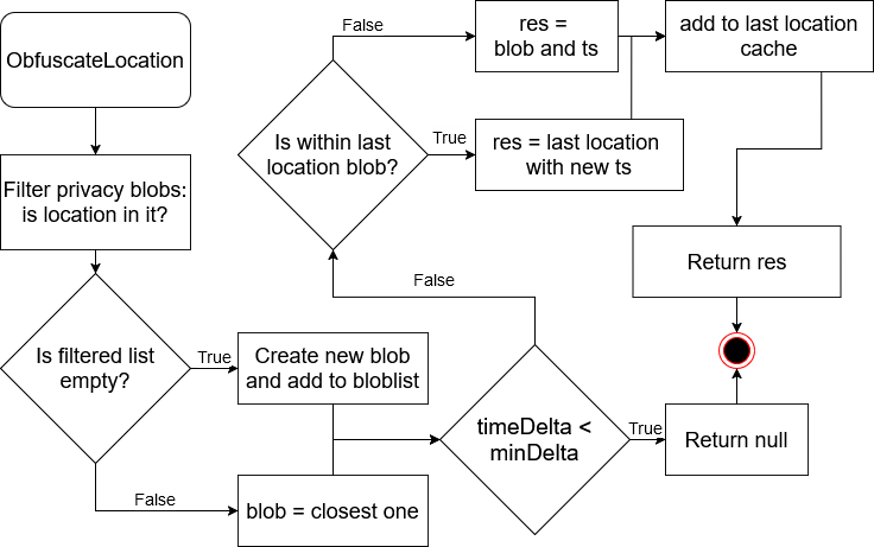
\includegraphics[width=0.75\textwidth]{images/obfuscatie_flow.png}
    \caption{Flow diagram van het obfuscatie algoritme}
    \label{fig:flow_obfuscatie_algoritmen}
\end{figure}
\subsection{Opslag}
Omdat veel obfuscatie-algoritmes permanente opslag nodig hebben moet iedere obfuscatieklasse ook een load en store functie implementeren. Dit heeft als argument de filesDir van de hoofdactiviteit. Dit is een object waarmee de developer de opslag van de applicatie kan beïnvloeden. In de standaardimplementatie wordt dit gebruikt om voorgaande privacy cirkels op te slaan in een voor andere applicaties afgesloten file. \cite{android_opslag}
\subsection{Netwerk}
De library heeft geen functionaliteit voor de locatie door te sturen naar een \gls{api} endpoint. Dit moet geïmplanteerd worden in de callback function die de developer meegeeft aan de LocationManager. In de testapplicatie word de library, aanbevolen door Android zelf, okhttp gebruikt om de locatie door te sturen.

\section{Applicatie}
De testapplicatie is ontworpen om de werking van de library te demonstreren en te testen, zoals geïllustreerd in Figuur~\ref{fig:applicatie}. De gebruikersinterface bestaat uit verschillende instellingen en knoppen die direct gekoppeld zijn aan de functionaliteit van de \texttt{LocationManager} en de locatieobfuscator.

De eerste vier instellingen betreffen de configuratie van de locatieverzameling:
\begin{itemize}
    \item \textbf{Priority:} Bepaalt de nauwkeurigheid en het energieverbruik van de \texttt{FusedLocationProvider}.
    \item \textbf{Foreground:} Geeft aan of de locatieverzameling als foreground service (met notificatie) of als background task wordt uitgevoerd.
    \item \textbf{Interval (ms):} Stelt het tijdsinterval in tussen opeenvolgende locatieverzoeken aan de \texttt{FusedLocationProvider}. Dit interval heeft geen invloed op het interval van de standaard locatieobfuscator.
    \item \textbf{Max runtime (min):} Bepaalt de maximale duur van de background service. Volgens de beperkingen van Android kan deze maximaal 10 minuten per 15 minuten actief zijn.
\end{itemize}

Daarnaast zijn er twee instellingen specifiek voor de standaardimplementatie van de locatieobfuscator:
\begin{itemize}
    \item \textbf{Blob radius:} De maximale straal van een privacycirkel.
    \item \textbf{Time between privacy:} De minimale tijd tussen het versturen van opeenvolgende locaties.
\end{itemize}

Onder de instellingen bevinden zich zes knoppen met de volgende functies:
\begin{itemize}
    \item \textbf{Permissies aanvragen:} De eerste twee knoppen vragen de benodigde permissies op bij de gebruiker. De status van deze permissies wordt weergegeven en geüpdatet via LiveData zoals te zien in de tweede screenshot.
    \item \textbf{Clear obfuscator storage:} Hiermee wordt de permanente opslag van de obfuscator gewist, zodat testen telkens met een schone lei kunnen starten.
    \item \textbf{Nieuwe UUID genereren:} Hiermee wordt een unieke identificatie gegenereerd voor elke test, zodat resultaten eenvoudig te onderscheiden zijn.
    \item \textbf{Tracking starten/stoppen:} De laatste twee knoppen zijn voor locatieverzameling. De status van de tracking wordt eveneens via LiveData weergegeven in de linker knop, zodat de interface altijd de actuele status toont.
\end{itemize}
In het onderste tekstvak worden de resultaten gelogd die via de callback (niet de debug-callback) worden doorgegeven. Dit biedt tijdens het testen een directe indicatie dat de applicatie actief locaties verwerkt.

De drie screenshots tonen respectievelijk:
\begin{itemize}
    \item De initiële opstart van de applicatie zonder verleende permissies.
    \item De situatie waarin de permissieknoppen de status van verleende permissies weergeven.
    \item De applicatie tijdens actieve tracking, waarbij een locatie is gelogd in het tekstvak.
\end{itemize}
\begin{figure}[h]
    \centering
    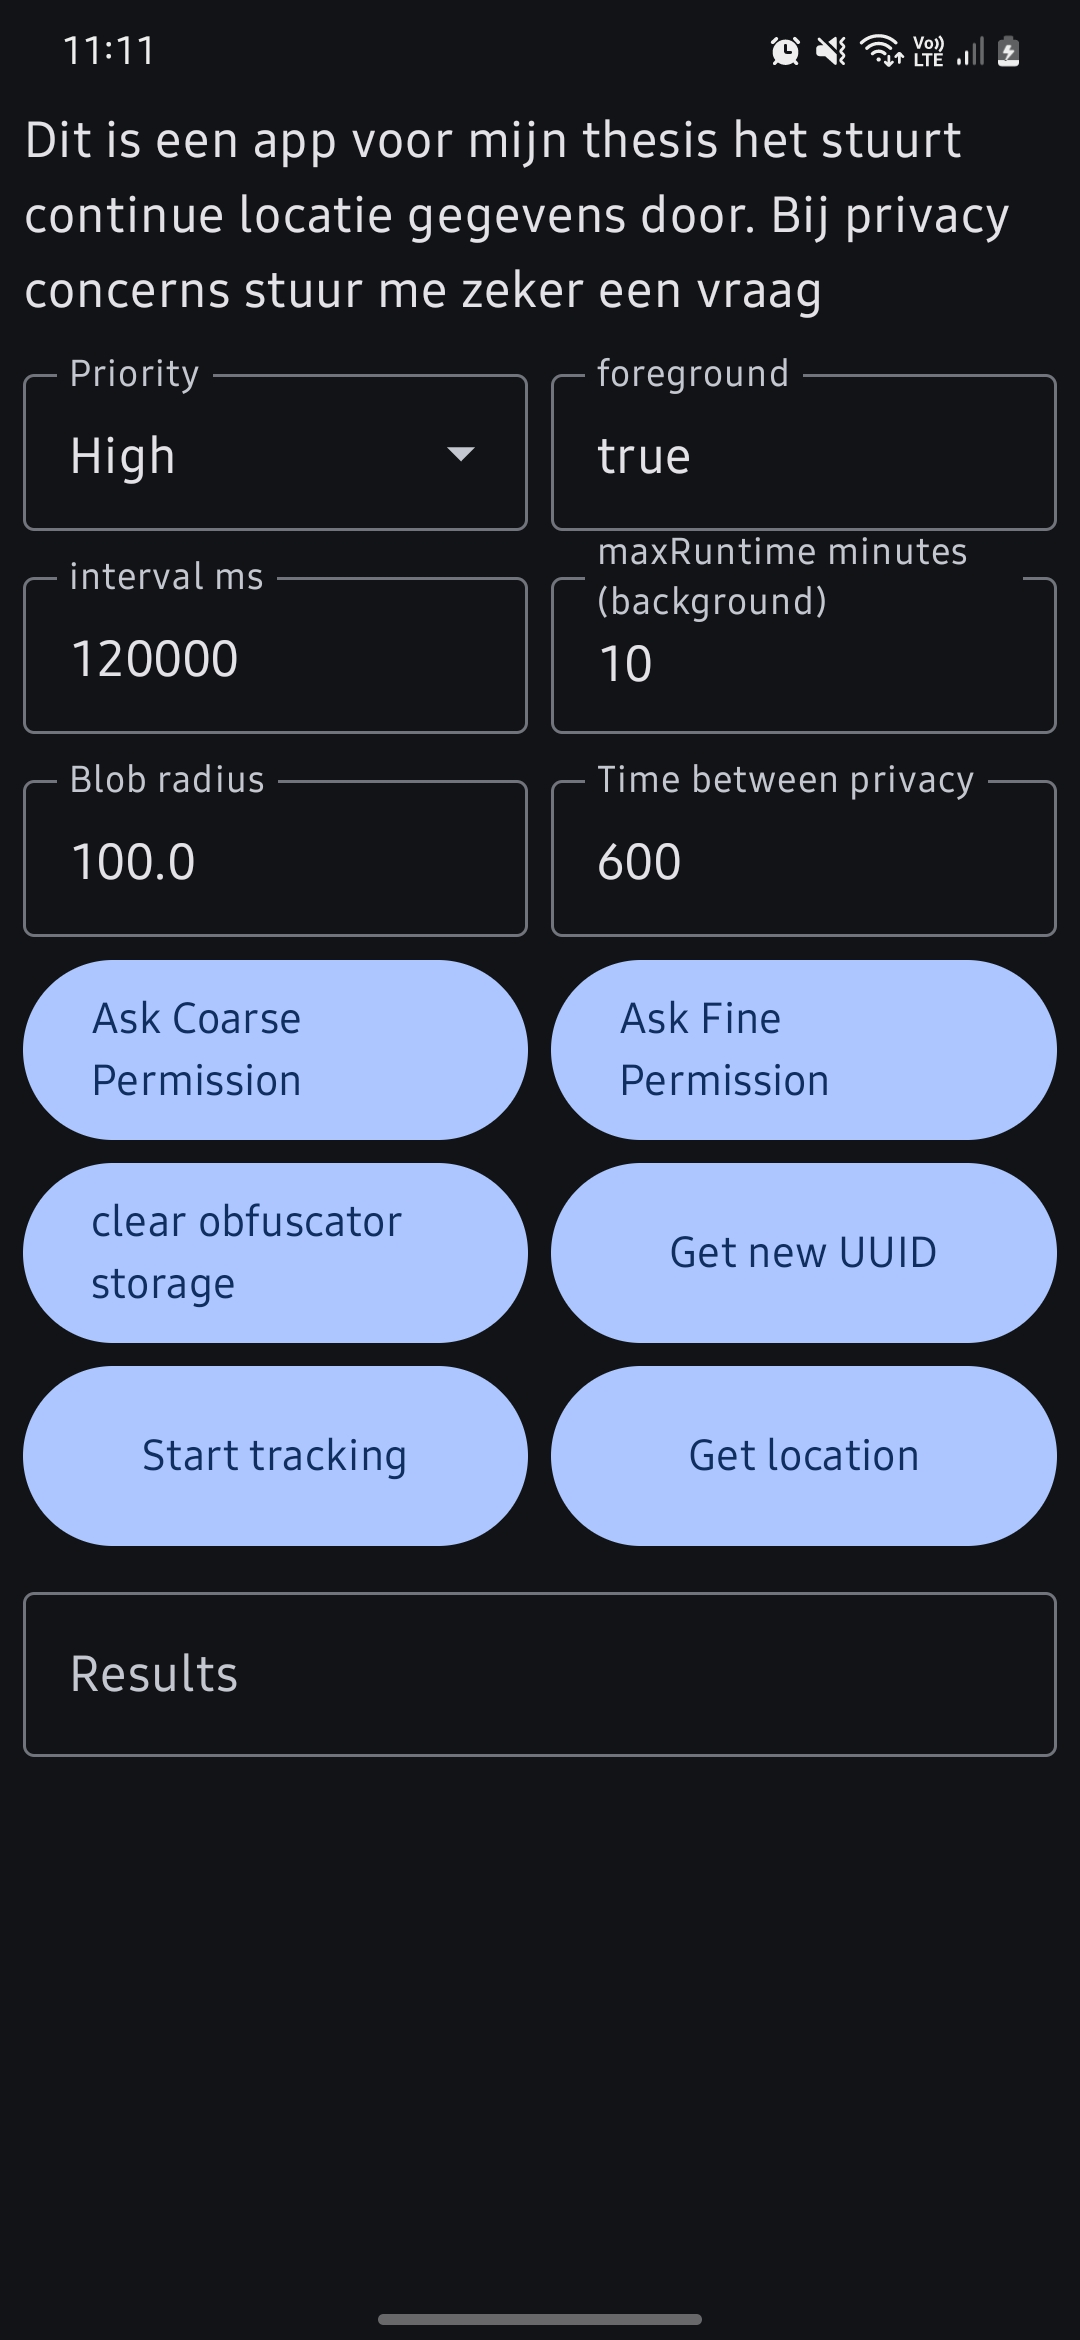
\includegraphics[width=0.32\textwidth]{images/screenshot_init.jpg}
    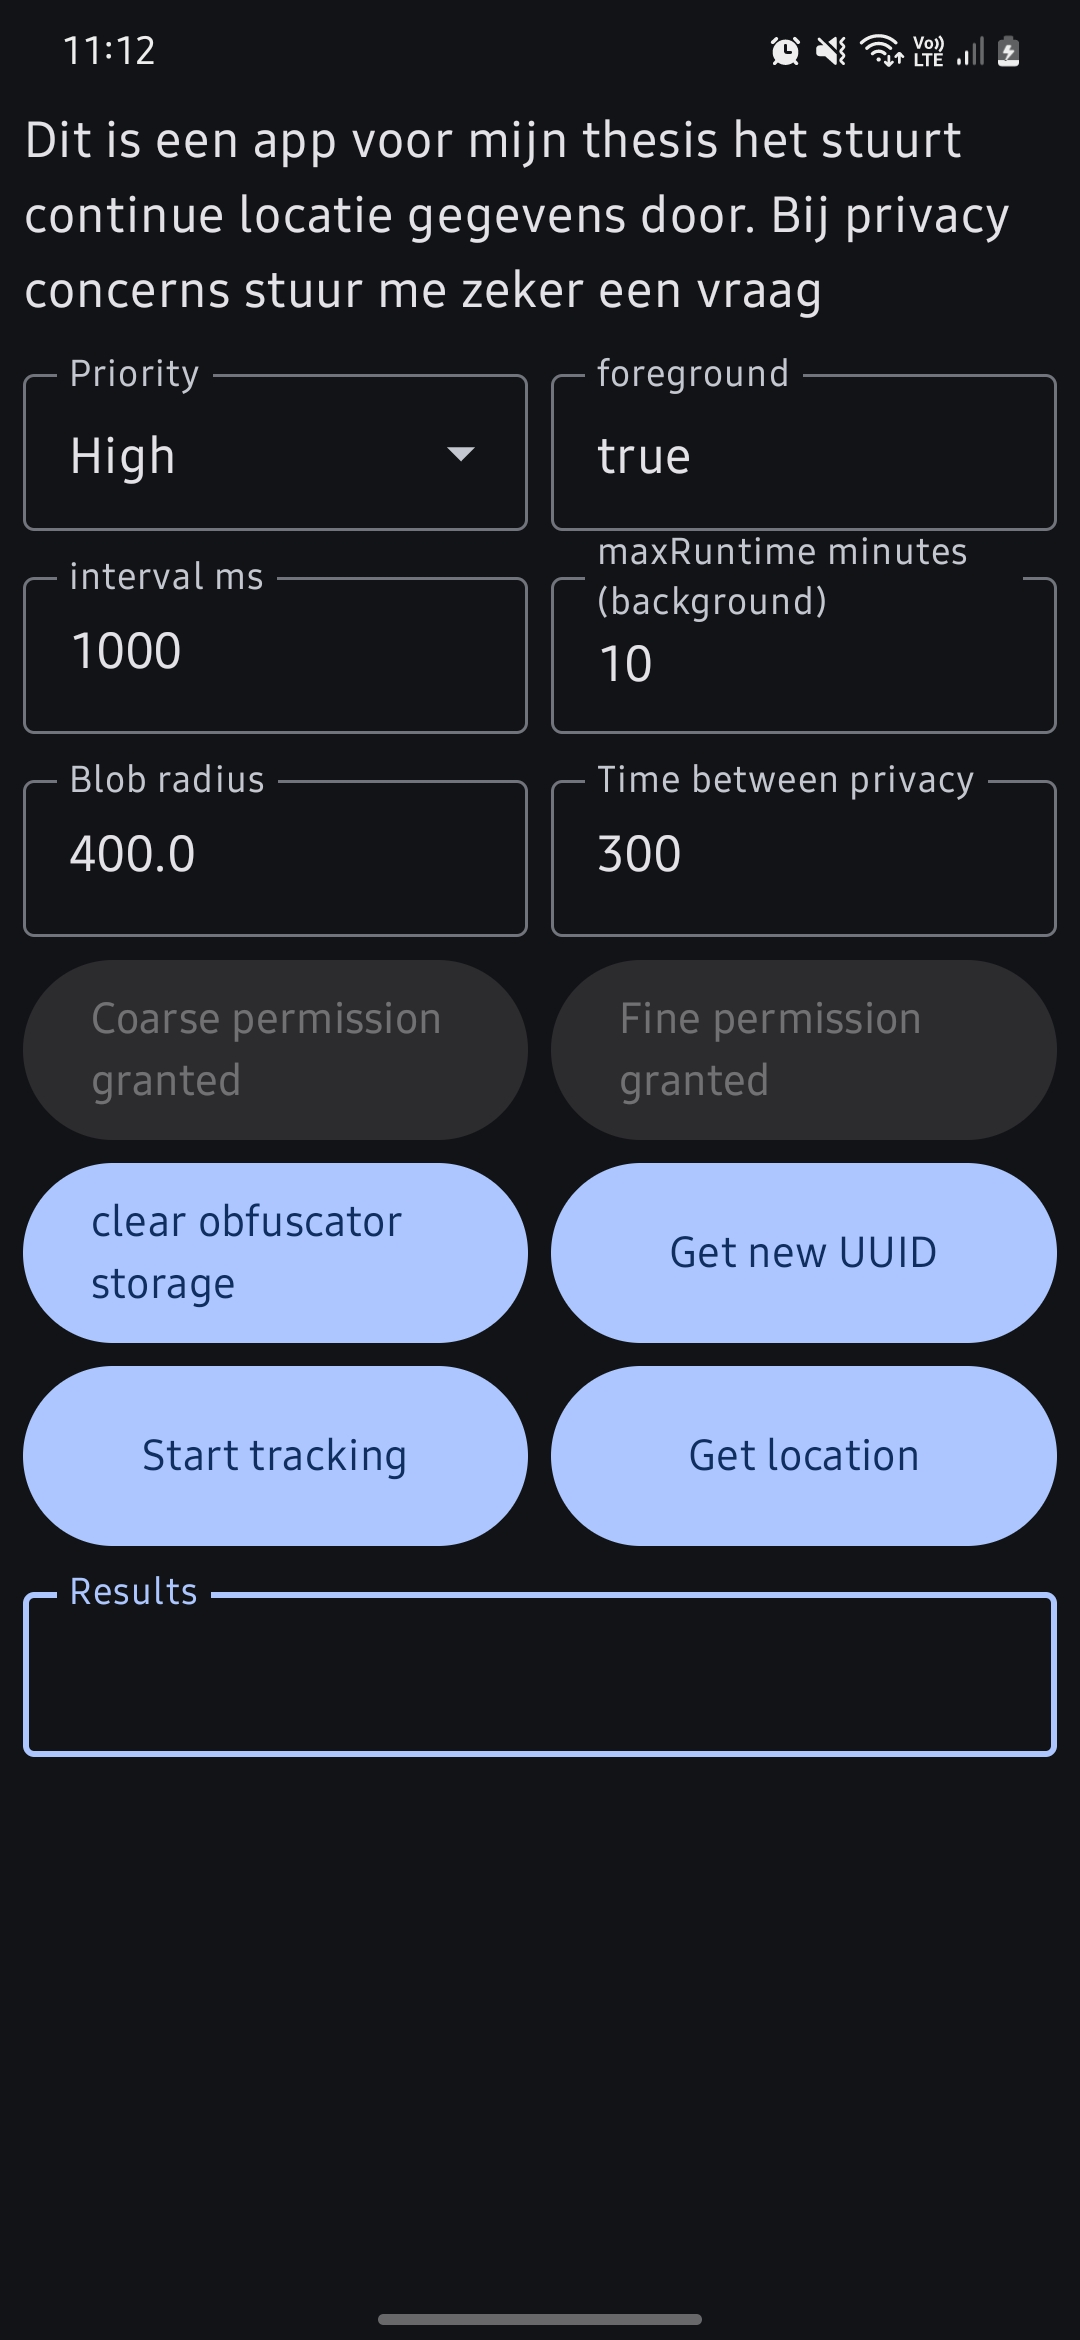
\includegraphics[width=0.32\textwidth]{images/screenshot_instellingen.jpg}
    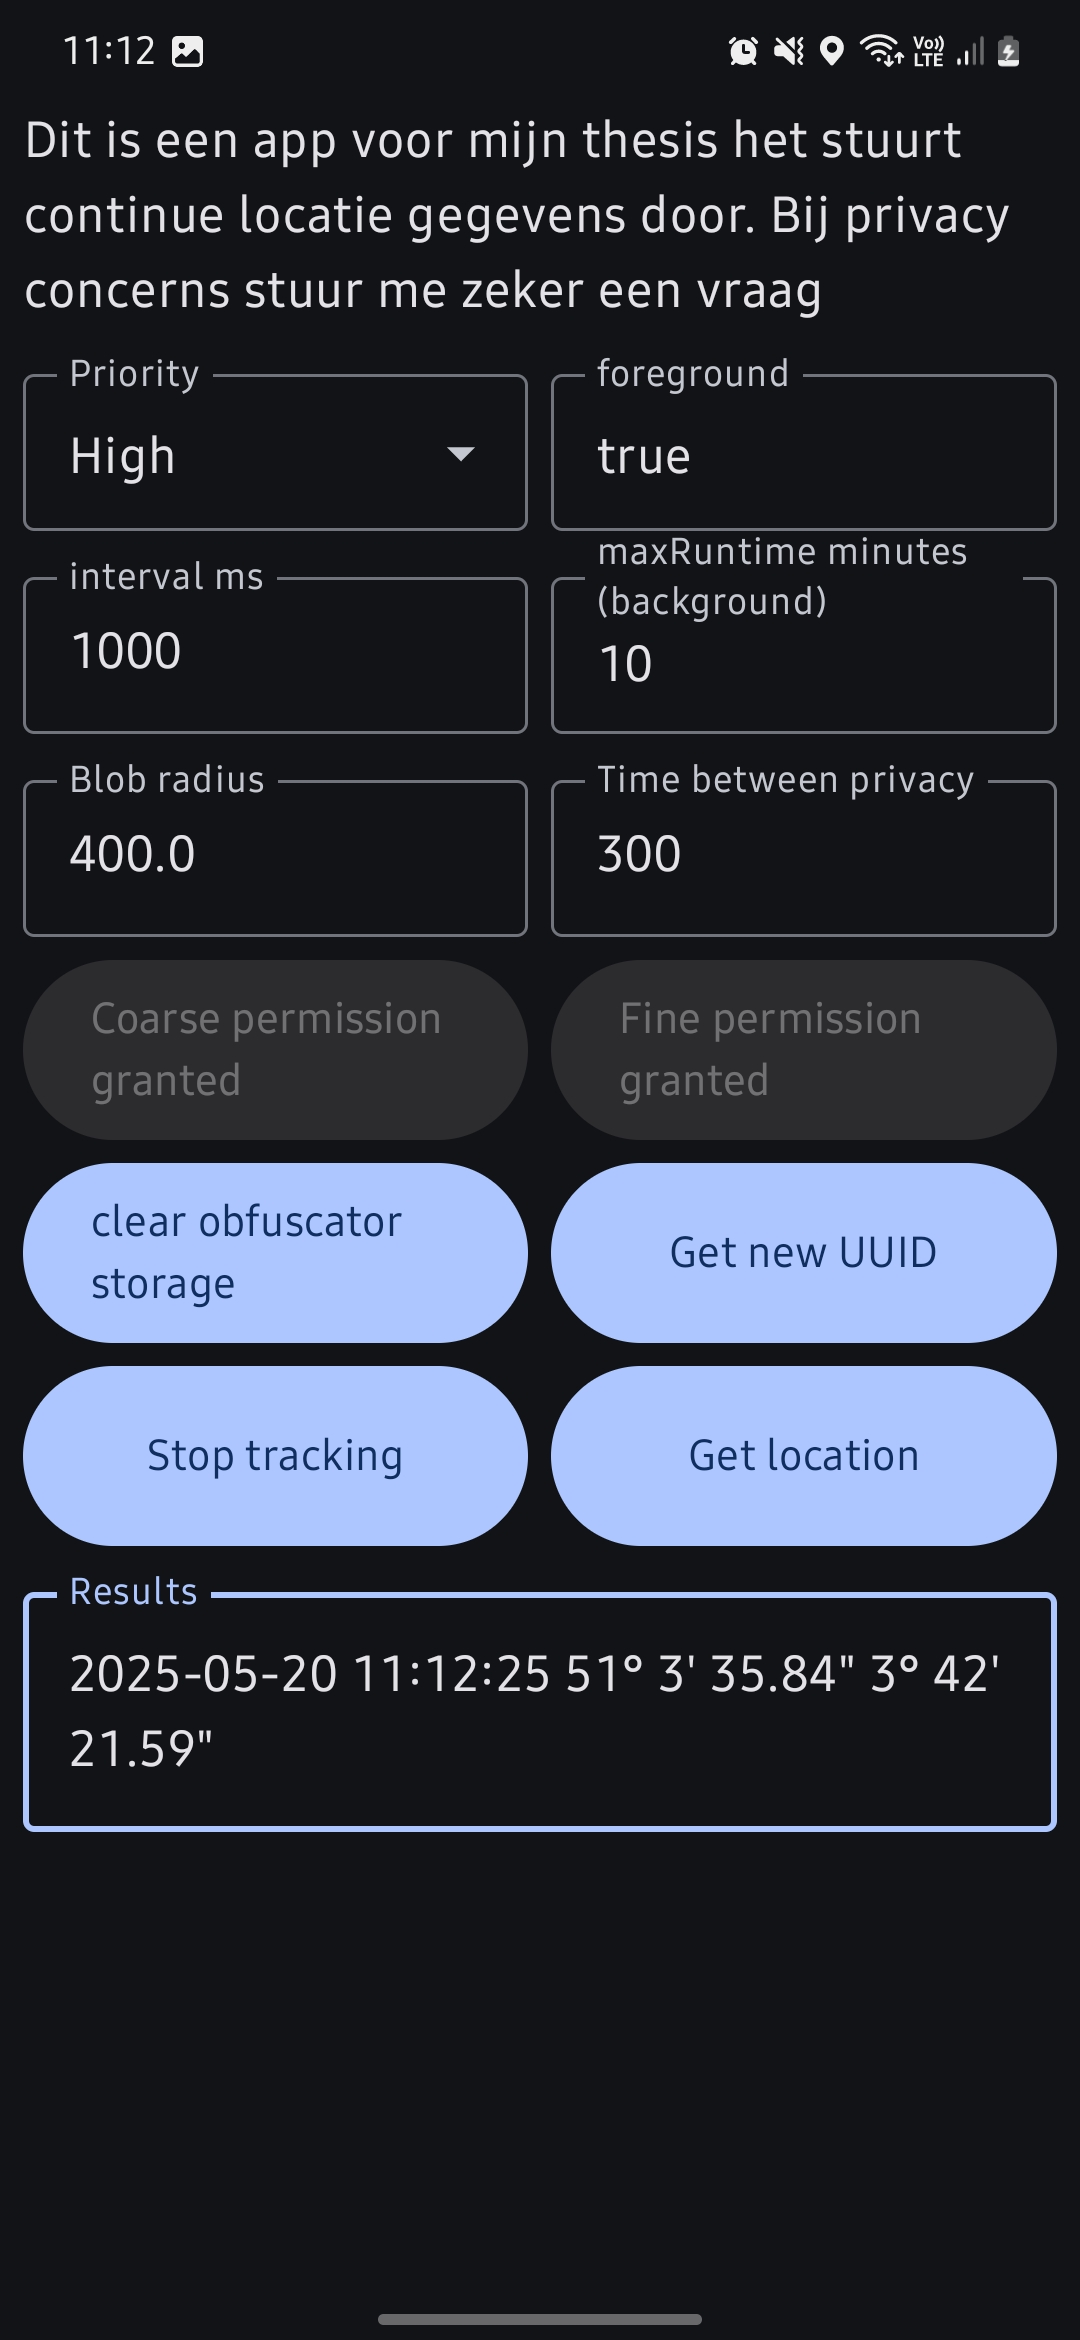
\includegraphics[width=0.32\textwidth]{images/screenshot_running.jpg}
    \caption{Visualisatie van de test applicatie}\label{fig:applicatie}
\end{figure}
\section{Dataverwerking}
\subsection{Verzameling}
Voor de verzameling van data werd gebruik gemaakt van een Azure-webserver, specifiek opgezet voor studenten, met twee endpoints: \texttt{location} en \texttt{blobs}. 

De \texttt{location}-endpoint ontving zowel de geobfusceerde als de originele locatiegegevens, afkomstig van de debug-callback, samen met relevante configuratieparameters. Deze gegevens werden opgeslagen in een CSV-bestand voor latere analyse. 

De \texttt{blobs}-endpoint werd gebruikt om de privacycirkels door te sturen. 

Om de afhankelijkheid van een continue internetverbinding te minimaliseren, werd een mechanisme geïmplementeerd waarbij de data lokaal werd opgeslagen wanneer er geen netwerkverbinding beschikbaar was. Zodra de verbinding werd hersteld, werden de opgeslagen gegevens alsnog doorgestuurd naar de server.
\subsection{Verwerking}
Voor de verwerking van de resultaten werden jupyter notebooks gehanteerd samen met de library Folium \cite{folium} om de resultaten visueel te kunnen representeren. 
In elke notebook is er een functie die de data inleest en locatiepunten die in de buurt van mijn privélocaties/privésfeer zijn weg filtert. Dit zorgt ervoor dat alle gevisualiseerde data gepubliceerd kan worden.
De eerste visualisatie was het verschil tussen coarse en fine Permissies vergelijken voor een experiment. Dit was beide op balanced power accuracy gebeurd zodat beide geen \gls{gps} satellieten gebruikt. Het resultaat is te zien in het hoofdstuk experimenten in state of the art \ref{fig:coarsevsfine1}\ref{fig:coarsevsfine2}.
Een tweede test betrof het gebruik van twee telefoons met coarse permissies en twee met fine permissies. Voor elk paar werd één telefoon ingesteld op high accuracy en de andere op balanced power accuracy. Deze test werd echter niet opgenomen in het preliminaire experimentenonderdeel van het hoofdstuk \textit{State of the Art}, omdat er te veel externe factoren waren die de resultaten beïnvloedden, zoals bv. de beperkingen opgelegd door de energiebesparingsfunctionaliteiten van Android.

De overige tests richtten zich op het evalueren van de standaardimplementatie van het obfuscatie-algoritme in de library. Hierbij werden verschillende variabelen gevarieerd om de werking van het algoritme te analyseren en mogelijke verbeterpunten te identificeren. De inzichten die uit deze tests voortkwamen, werden gebruikt om de library verder te debuggen en te optimaliseren. Een uitgebreide bespreking van deze resultaten is te vinden in het hoofdstuk \textit{Experimenten en resultaten}.

\section{Conclusie}
In dit hoofdstuk werd de implementatie van de Android-library uitgebreid besproken. De library is ontworpen om locatiegegevens op een privacyvriendelijke manier te verzamelen en te verwerken. Het centrale beheer van locatieverzameling wordt uitgevoerd door de \texttt{LocationManager}, terwijl de WorkManager zorgt voor een flexibele en betrouwbare uitvoering van zowel foreground services als periodieke background tasks.

De library integreert een standaard obfuscatie-algoritme gebaseerd op privacycirkels, waarmee gevoelige informatie effectief wordt beschermd. Ontwikkelaars hebben de mogelijkheid om aangepaste obfuscatieklassen te implementeren en gebruik te maken van debug-callbacks voor analyse. Permanente opslag wordt ondersteund om privacycirkels en andere gegevens veilig te bewaren.

Daarnaast werd een testapplicatie ontwikkeld om data te verzamelen via een Azure-webserver. Hierbij werden mechanismen geïmplementeerd om gegevens lokaal op te slaan bij netwerkuitval, wat de betrouwbaarheid van de oplossing verhoogt. Deze aanpak minimaliseert de afhankelijkheid van een continue internetverbinding.

